% ==================================================
% Section 6
% ==================================================
\section{Sampling-Time Effect and Tustin Redesign}

The discrete-time controller of Section~5 used the simplest approximations: the
error derivatives were computed with backward differences and the adaptation law
was integrated using a discrete-time update.

\subsection{Performance Degradation with Increasing Sampling Time}

Figure~\ref{fig:s6_degradation} shows the tracking error \(e(t)\) and the
filtered error \(z(t)\) for \(T_s\) from \(0.01\) to \(0.05~\mathrm{s}\). As seen below, the peak
tracking error grows as \(T_s\) increases.

\begin{figure}[H]
\centering
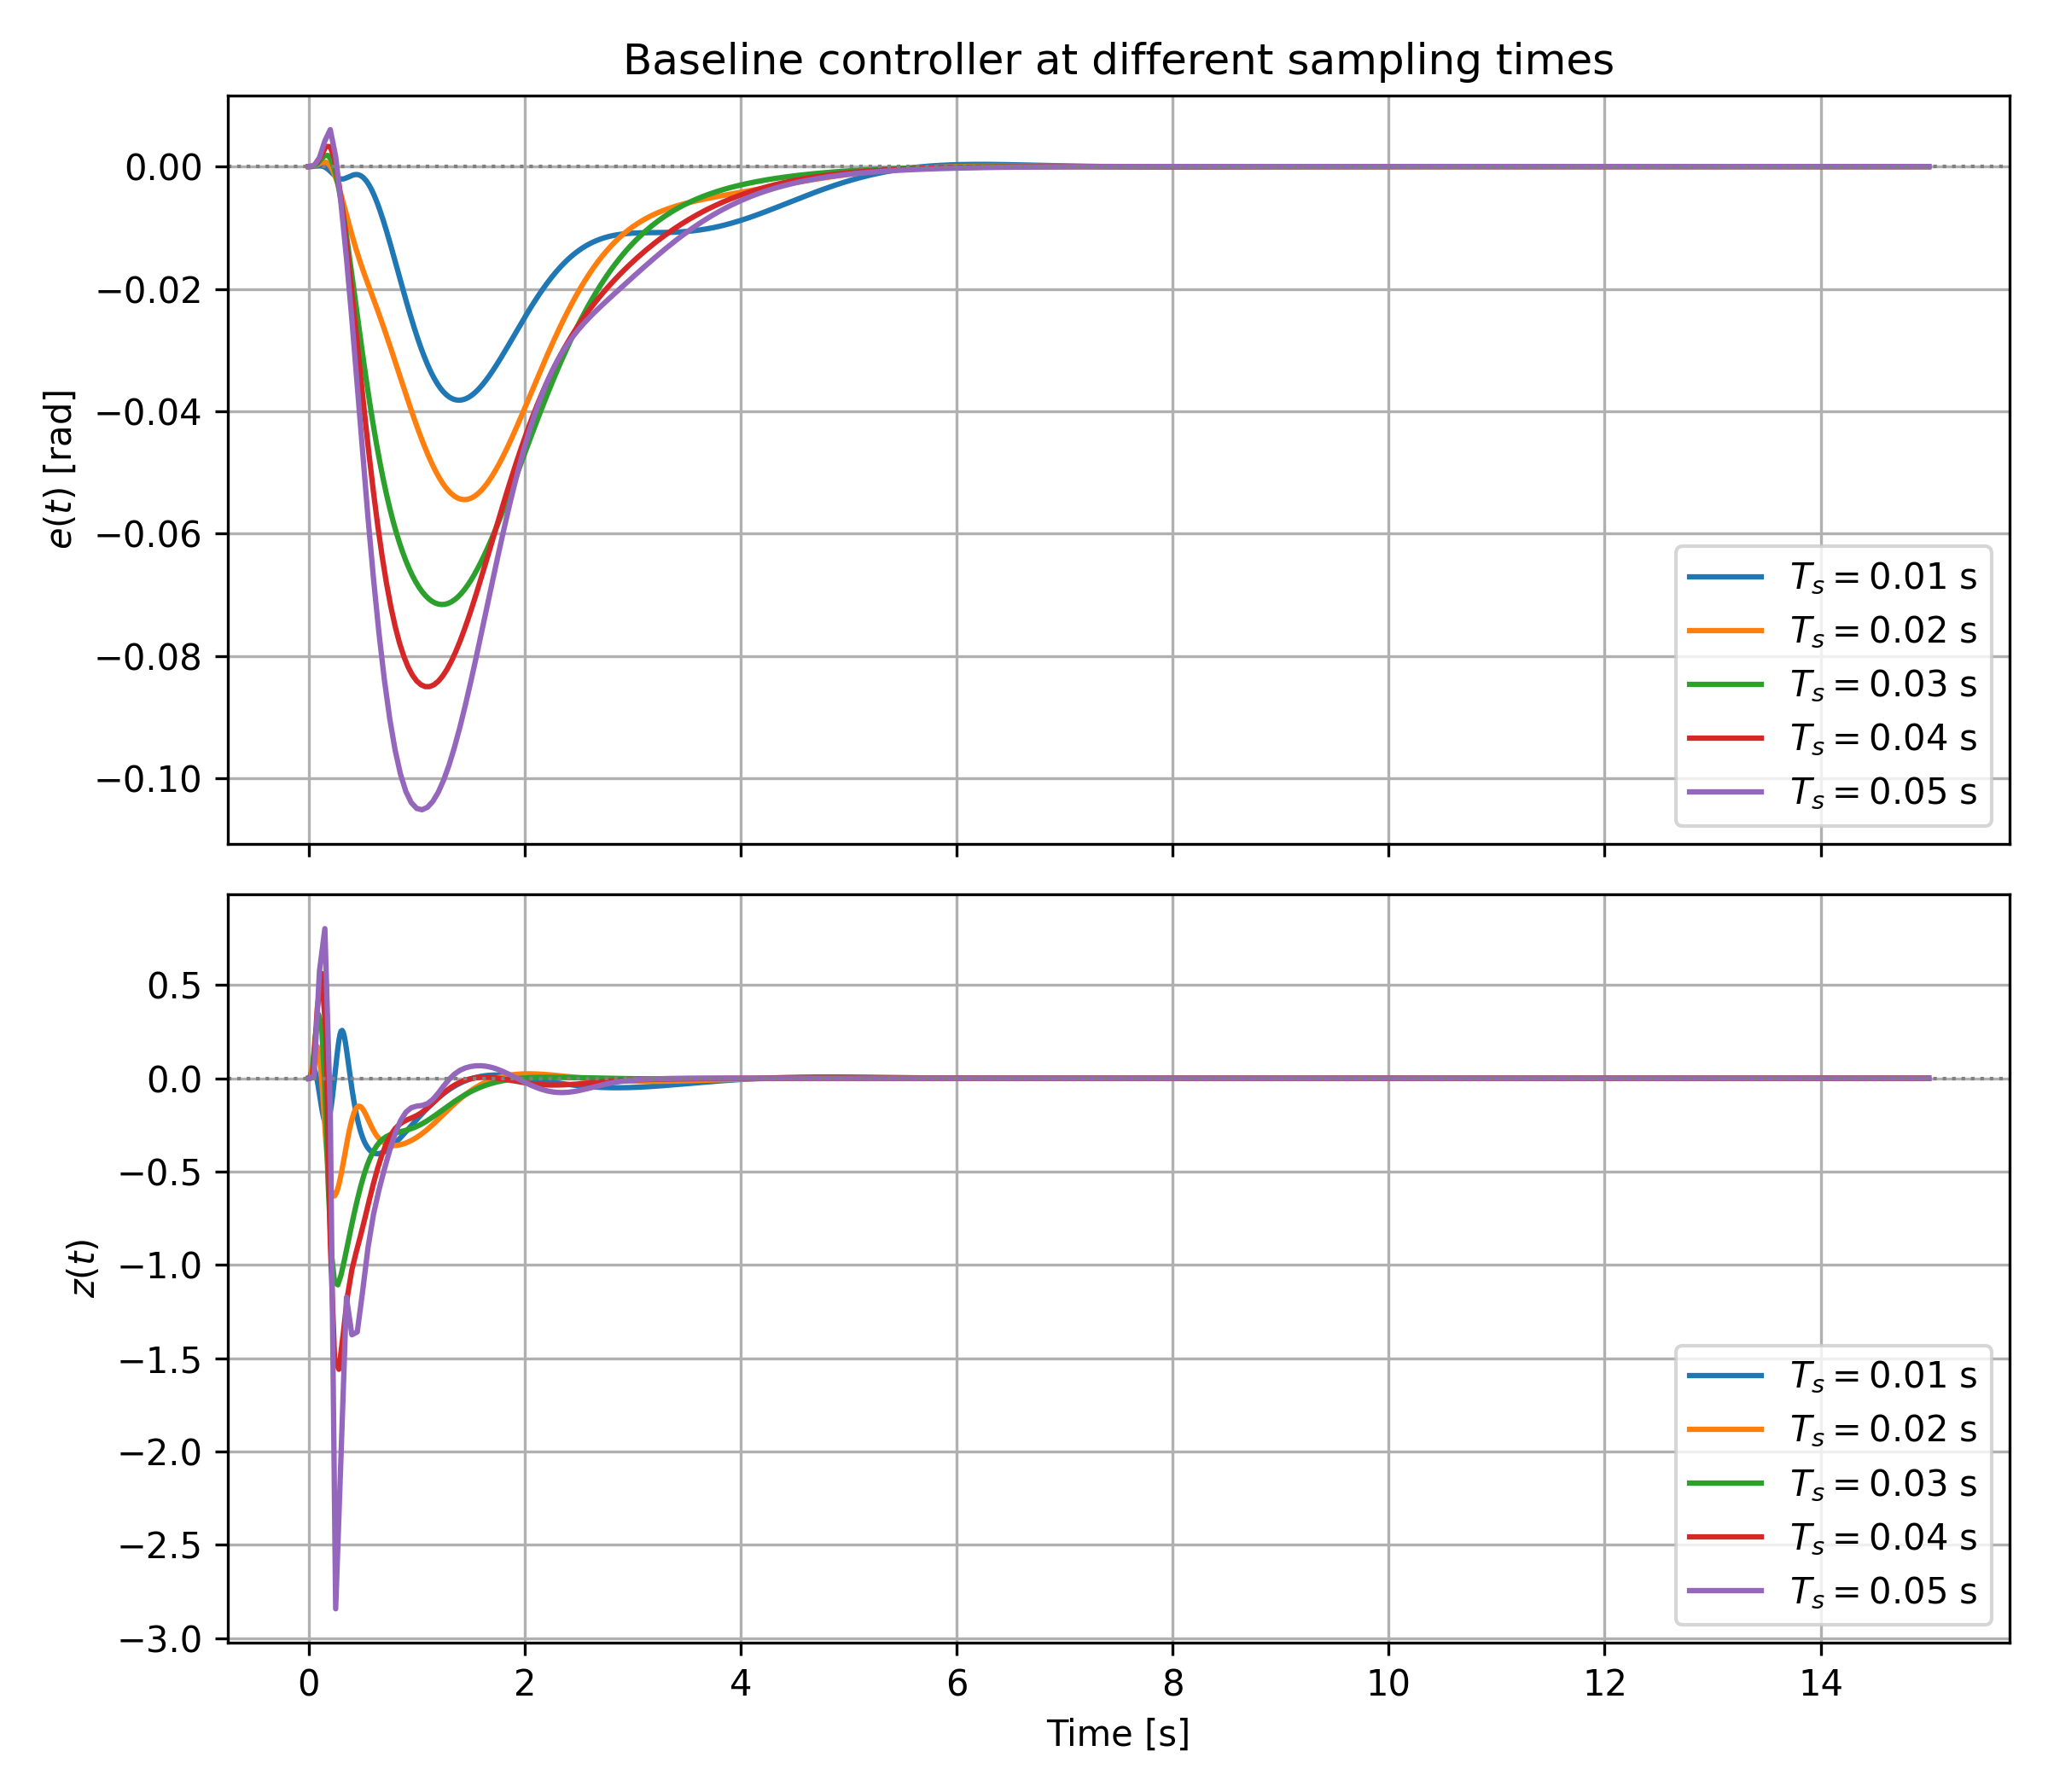
\includegraphics[width=0.7\textwidth]{figs/hw/section6_degradation.png}
\caption{Tracking error \(e(t)\) (top) and
filtered error \(z(t)\) (bottom) for increasing sampling periods.}
\label{fig:s6_degradation}
\end{figure}

\noindent As the sampling period \(T_s\) increases, the backward-difference approximations in~\eqref{eq:discrete_bd} become less accurate. The first derivative is approximated using a term proportional to \(1/T_s\), while the second derivative uses a term proportional to \(1/T_s^2\). Because the controller depends on both derivatives, the discretization error becomes more significant as the sampling interval increases.
As a result, the computed control input gradually deviates from its continuous-time tracking. For sampling periods of approximately \(T_s=0.06~\mathrm{s}\) and above, the closed-loop system loses stability and diverges. The discrete-time update used for the adaptation law also introduces discretization error, although its effect is smaller than that of the derivative approximations.

\subsection{Improved Design - Tustin Discretizations}

The results of the previous section showed that the performance degradation is mainly caused by the numerical errors introduced by the backward-difference approximation as the sampling period increases. To achieve good performance without reducing \(T_s\), the controller is re-discretized using the Tustin discretizations:
\begin{equation}
s
\;\longleftarrow\;
\frac{2}{T_s}\,
\frac{z-1}{z+1}
\label{eq:s6_tustin}
\end{equation}
which provides a more accurate approximation of the continuous-time dynamics than simple methods. The backward-difference approximation used in the baseline controller becomes less accurate as the sampling period increases. To improve the derivative estimation, the error derivatives are computed using a first-order filtered derivative. Applying the Tustin transformation to the filter gives:
\begin{equation}
\dot{\hat{e}}[k]=
\frac{
a\left(e[k]-e[k-1]\right)
-
\left(1-\tau_f a\right)\dot{\hat{e}}[k-1]
}
{\tau_f a+1},
\qquad
a=\frac{2}{T_s}
\label{eq:s6_dirty}
\end{equation}
where \(\tau_f\) is the derivative filter time constant. The second derivative is obtained by applying the same filtered-derivative calculation to \(\dot{\hat{e}}[k]\). This provides smoother derivative estimates and reduces the sensitivity of the controller to larger sampling periods. The adaptation law is also discretized using the Tustin method instead of the discrete-time update approximation. The resulting update equation is:
\begin{equation}
\hat{\theta}[k]
=
\hat{\theta}[k-1]
-
\frac{T_s}{2}\,
\Gamma
\left(
\phi[k]z[k]
+
\phi[k-1]z[k-1]
\right).
\label{eq:s6_trap}
\end{equation}
This update uses both the current and previous samples, providing a more accurate approximation of the continuous-time adaptation law. The remaining controller calculations are performed as in Section~5.

\subsection{Simulation Results}

Figure~\ref{fig:s6_fix} compares the baseline and redesigned controllers for
$T_s=0.05~\mathrm{s}$. The figure shows both the output
tracking and the corresponding tracking error for step input.

\begin{figure}[H]
\centering
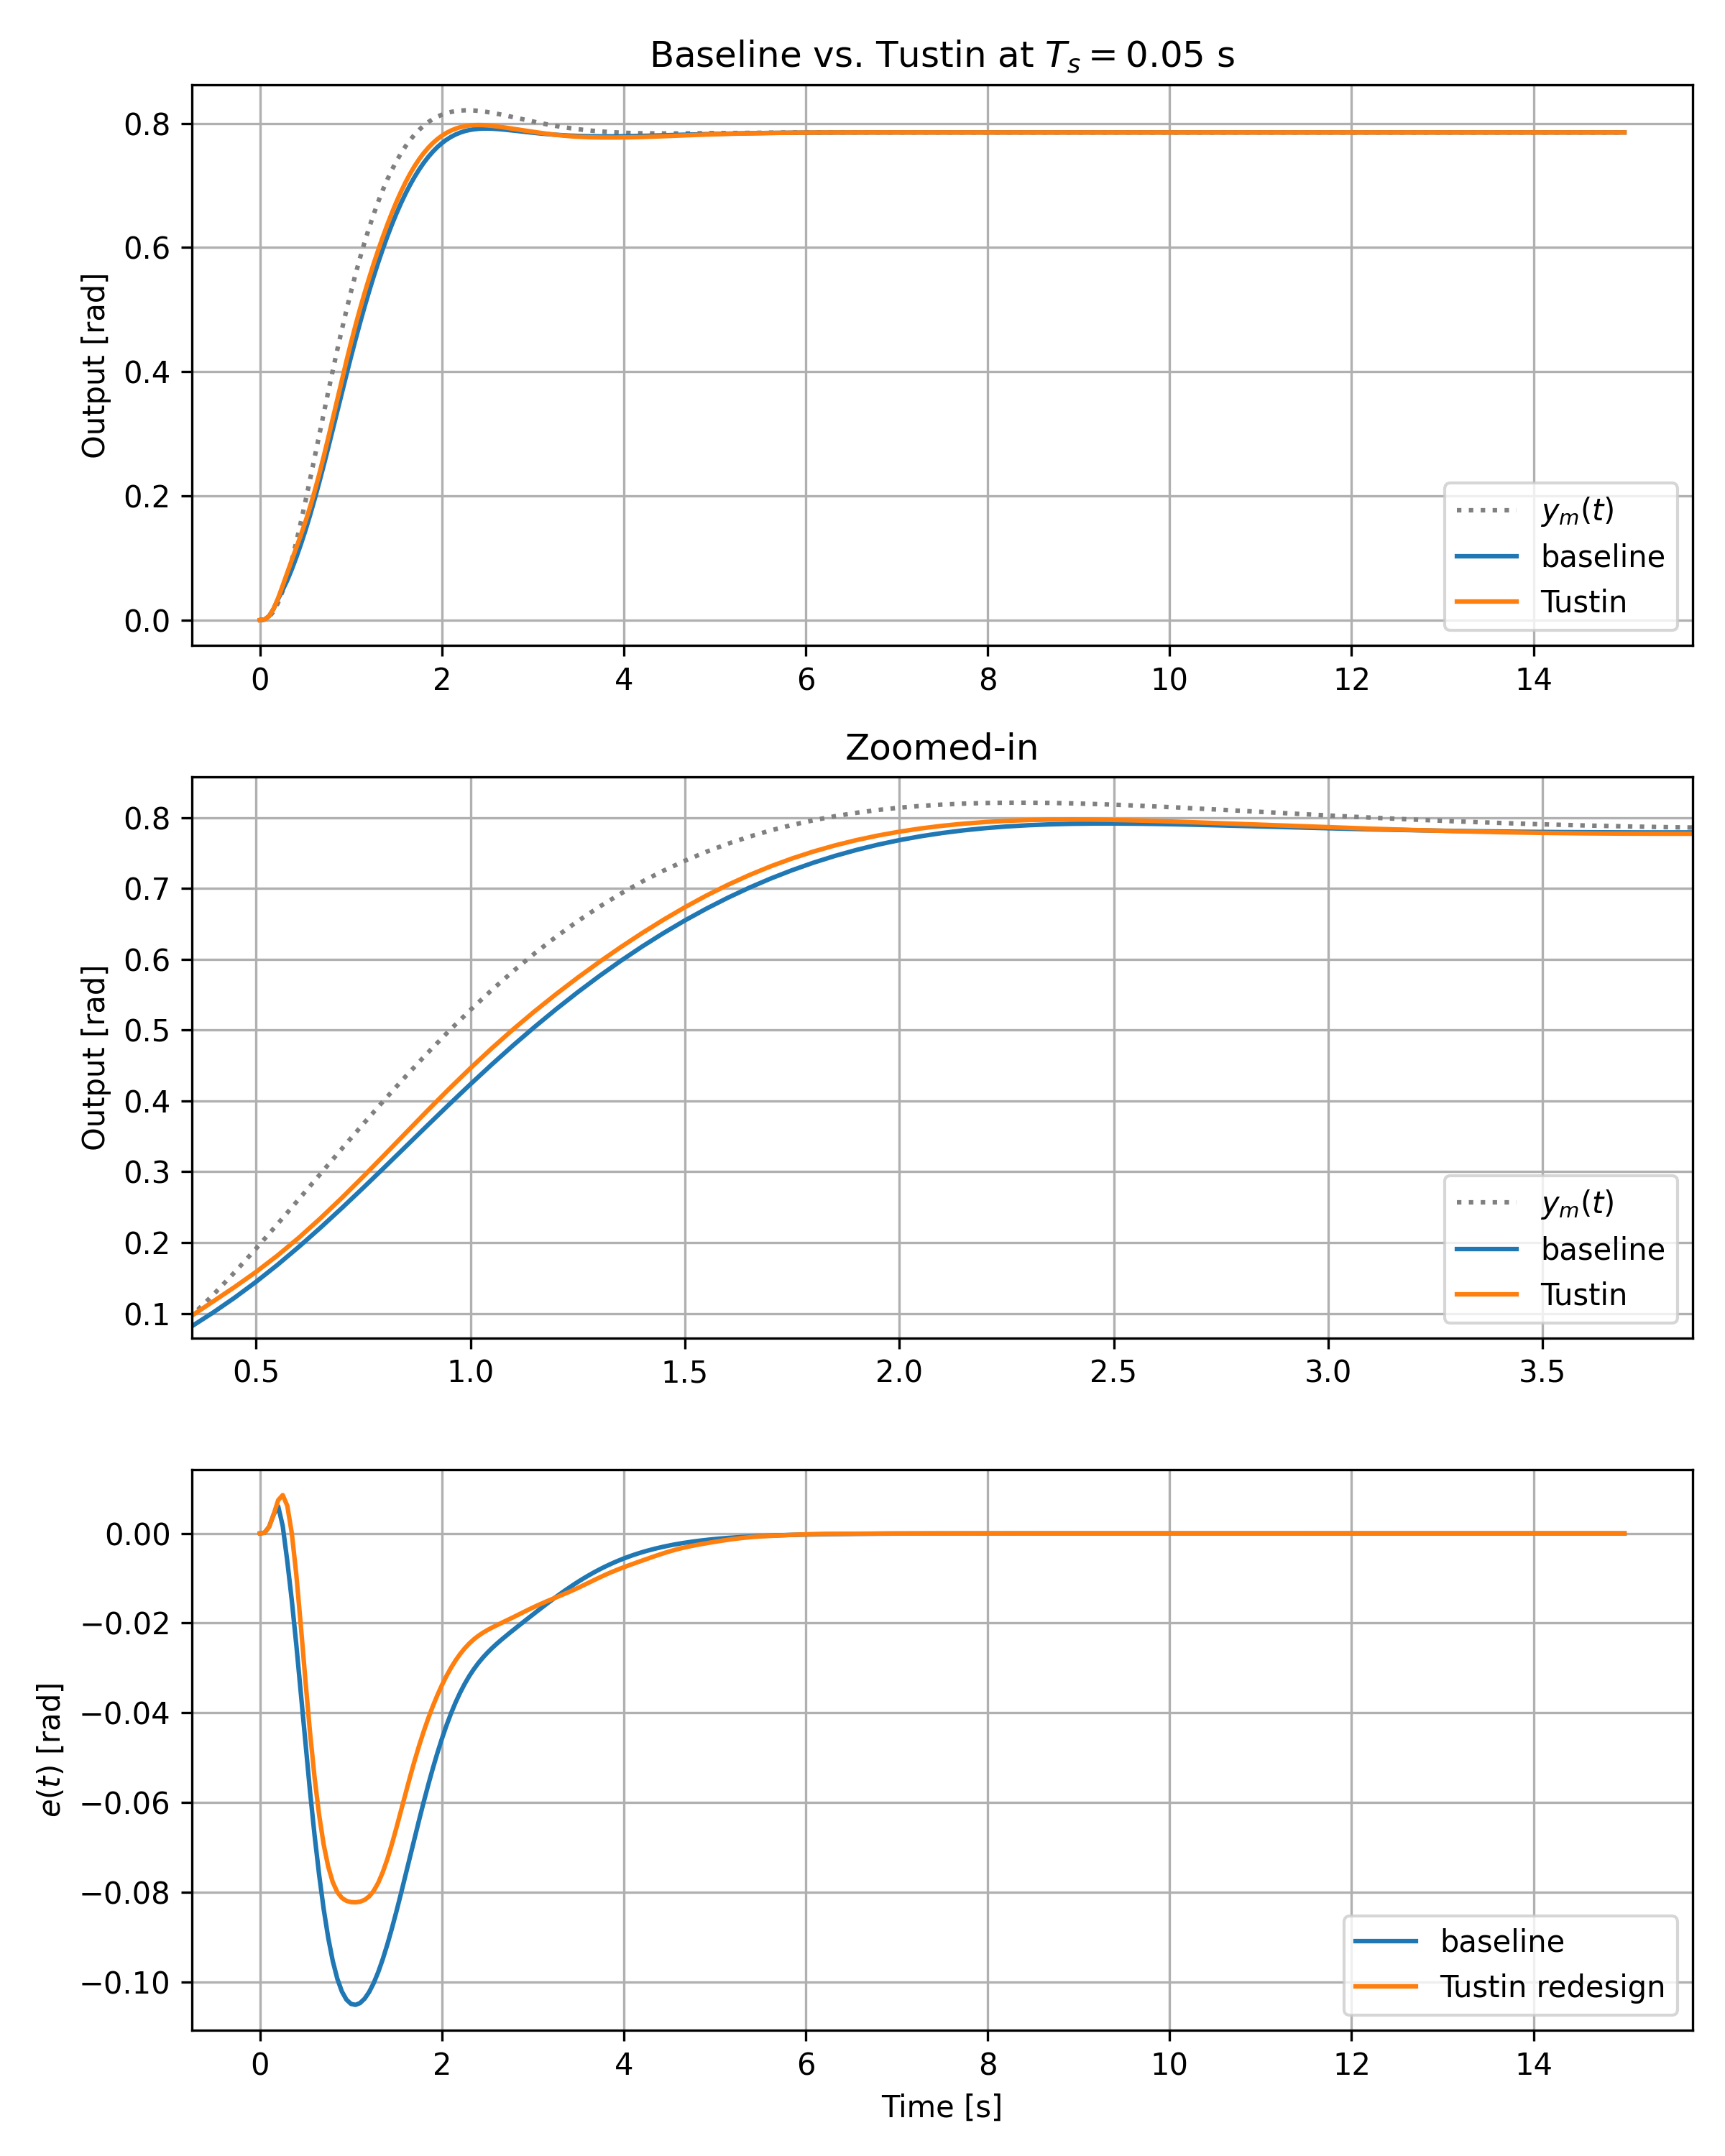
\includegraphics[width=0.7\textwidth]{figs/hw/section6_tustin_fix.png}
\caption{Output tracking
(top) and tracking error (bottom) for the baseline and Tustin-based
controllers.}
\label{fig:s6_fix}
\end{figure}

\noindent The redesigned controller shows improved transient performance, smaller peak tracking error than the baseline implementation, and faster convergence to the reference model.
The tracking error also smaller, indicating that the controller
better preserves the behavior of the original continuous-time design. Overall, the Tustin-based implementation successfully
reduces the performance degradation caused by the discrete-time realization and
allows the controller to operate better with larger sampling periods.

\bigskip